\documentclass[11pt,a4paper]{article}

\usepackage[margin=1in]{geometry}
\usepackage{graphicx}
\usepackage{booktabs}
\usepackage{array}
\usepackage{longtable}
\usepackage{caption}
\usepackage{subcaption}
\usepackage{xcolor}
\usepackage{listings}
\usepackage{amsmath}
\usepackage{enumitem}
\usepackage{fancyhdr}
\usepackage{titlesec}
\usepackage[hidelinks]{hyperref}

\definecolor{codebg}{RGB}{245,245,245}
\definecolor{codekw}{RGB}{0,80,150}
\definecolor{codecomment}{RGB}{110,110,110}
\definecolor{codestring}{RGB}{140,20,20}

\lstset{
  backgroundcolor=\color{codebg},
  basicstyle=\ttfamily\small,
  keywordstyle=\color{codekw}\bfseries,
  commentstyle=\color{codecomment}\itshape,
  stringstyle=\color{codestring},
  showstringspaces=false,
  breaklines=true,
  frame=single,
  rulecolor=\color{gray!40},
  numbers=left,
  numberstyle=\tiny\color{gray},
  xleftmargin=1.8em,
  language=Python
}

\titleformat{\section}{\normalfont\Large\bfseries}{\thesection}{1em}{}
\titleformat{\subsection}{\normalfont\large\bfseries}{\thesubsection}{1em}{}

\pagestyle{fancy}
\fancyhf{}
\fancyhead[L]{ICS1512 -- Machine Learning Algorithms Laboratory}
\fancyhead[R]{Experiment 6}
\fancyfoot[C]{\thepage}
\renewcommand{\headrulewidth}{0.4pt}

\title{}
\date{}

\begin{document}

% ---------------- Title Page ----------------
\begin{titlepage}
\centering
\vspace*{1cm}
{\Large\bfseries Sri Sivasubramaniya Nadar College of Engineering, Chennai\par}
\vspace{0.2cm}
{\normalsize (An Autonomous Institution Affiliated to Anna University)\par}
\vspace{1.2cm}

{\Large\bfseries Machine Learning Algorithms Laboratory\par}
\vspace{0.3cm}
{\large ICS1512\par}
\vspace{1.5cm}

\begin{tabular}{|p{5.5cm}|p{7cm}|}
\hline
Degree \& Branch & M.Tech (Integrated) Computer Science \& Engineering \\
\hline
Semester & V \\
\hline
Academic Year & 2026--2027 (Odd) \\
\hline
Batch & 2024--2029 \\
\hline
\end{tabular}

\vspace{1.8cm}
{\Large\bfseries Experiment 6\par}
\vspace{0.3cm}
{\large Bagging, Boosting, and Stacked Ensemble Models\footnote{\textbf{GitHub Repository: }\url{https://github.com/VijayaraaghavanKS/ML}}\par}
\vspace{2.5cm}

\begin{tabular}{ll}
Submitted by: & \textbf{Vijayaraaghavan K S} \\[4pt]
Register Number: & \textbf{3122247001066} \\[4pt]
Year: & III Year \\[4pt]
Programme: & M.Tech Integrated, CSE \\[4pt]
Faculty: & Dr. Poreddy Ajay Kumar Reddy \\[4pt]
\end{tabular}

\vfill
\end{titlepage}

\tableofcontents
\newpage

% ==========================================================
\section{Aim and Objective}
To implement three ensemble learning strategies -- Bagging, Boosting, and a heterogeneous Stacked Ensemble -- on the Wisconsin Diagnostic Breast Cancer dataset, tune each with 5-fold cross-validated hyperparameter search, and analyze how each strategy trades off bias against variance relative to a single Decision Tree.

% ==========================================================
\section{Problem Statement}
The input is the same 30-dimensional vector of nuclear-morphology measurements used in Experiment 5 (radius, texture, perimeter, area, smoothness, and related shape descriptors, each summarized as a mean, standard error, and ``worst'' value); the output is a binary diagnosis, malignant or benign. Experiment 5 already showed that a single tuned Decision Tree and a Random Forest tie on test-set accuracy while the forest wins on cross-validated accuracy and stability. This experiment asks a broader question: given the same base learner (or a mix of different ones), which combination strategy -- parallel averaging (Bagging), sequential error correction (Boosting), or learned combination (Stacking) -- makes the best use of it, and does the answer differ depending on whether the goal is reducing variance, reducing bias, or exploiting model diversity?

% ==========================================================
\section{Theory}

\subsection{Bagging (Bootstrap Aggregation)}
Bagging trains many copies of a high-variance base model, each on an independent bootstrap resample of the training data, and combines their predictions by majority vote. Because the resamples differ, the individual models' errors are only weakly correlated, so averaging them cancels out a large share of their variance without changing their bias much. Bagging is most useful when the base learner is already low-bias but high-variance, which is exactly the profile of an unconstrained Decision Tree.

\subsection{Boosting}
Boosting trains base learners sequentially rather than independently: each new learner is fit to pay more attention to the samples the ensemble has gotten wrong so far (AdaBoost reweights misclassified samples before fitting the next learner; Gradient Boosting instead fits the next tree to the residual gradient of the loss function). This directly targets bias -- a boosted ensemble of weak learners can represent a far more complex decision boundary than any one of them individually -- though pushed too far (too many rounds, too high a learning rate) boosting can start to raise variance and overfit.

\subsection{Stacked Ensemble (Stacking)}
Stacking trains several heterogeneous base learners and a separate meta-learner that is trained on the base learners' out-of-fold predictions to learn how to best combine them. Unlike bagging and boosting, which typically use one type of base learner, stacking is explicitly designed to exploit diversity: base learners with different inductive biases (a margin-based SVM, a probabilistic Naive Bayes classifier, and an axis-aligned Decision Tree, in this experiment) tend to make different, less-correlated mistakes, giving the meta-learner more complementary signal to work with than a homogeneous ensemble would.

% ==========================================================
\section{Machine Learning Algorithm}

\subsection{Bagging Classifier}
\textbf{Working principle:} draw \texttt{n\_estimators} bootstrap samples (sampled with replacement, each of size \texttt{max\_samples} $\times$ training set) from the training data, fit an independent copy of the base estimator (a Decision Tree here) on each sample, restricting each fit to a random subset of \texttt{max\_features} columns, and combine the predictions by majority vote.
\textbf{Mathematical formulation:} for $B$ bootstrap models $T_1,\dots,T_B$, the ensemble prediction is $\hat y = \operatorname{mode}\{T_1(x),\dots,T_B(x)\}$; since each $T_b$ is trained on an independent resample, $\operatorname{Var}(\hat y) \approx \operatorname{Var}(T_b)/B$ under the (optimistic but directionally correct) assumption of independent errors, which is why more estimators generally reduces variance up to a point of diminishing returns.
\textbf{Advantages:} straightforward to parallelize since every base model trains independently, and it reliably reduces variance for any high-variance base learner without requiring any change to how that base learner is trained.
\textbf{Limitations:} it cannot fix a base learner that is systematically biased (averaging many equally wrong models does not make them right), and it loses the single-model's interpretability.

\subsection{Boosting (AdaBoost and Gradient Boosting)}
\textbf{Working principle:} AdaBoost starts with uniform sample weights, fits a weak learner, increases the weight of misclassified samples, and repeats, combining all learners in a weighted vote; Gradient Boosting instead fits each new tree to the negative gradient of the loss with respect to the current ensemble's predictions, effectively doing gradient descent in function space.
\textbf{Mathematical formulation:} AdaBoost's final prediction is $\hat y = \operatorname{sign}\left(\sum_{m=1}^M \alpha_m h_m(x)\right)$ where $\alpha_m = \frac{1}{2}\ln\frac{1-\epsilon_m}{\epsilon_m}$ weights each weak learner $h_m$ by its own weighted error rate $\epsilon_m$; Gradient Boosting builds $F_M(x) = F_0(x) + \sum_{m=1}^M \nu \cdot h_m(x)$ where each $h_m$ is fit to the residual gradient $-\partial L/\partial F_{m-1}$ and $\nu$ is the learning rate controlling each step's contribution.
\textbf{Advantages:} directly and iteratively reduces bias, so a boosted ensemble of shallow trees can fit decision boundaries a single shallow tree cannot; Gradient Boosting in particular tends to be very accurate on structured/tabular data such as this one.
\textbf{Limitations:} training is inherently sequential (harder to parallelize than bagging), it is more sensitive to noisy labels and outliers since it keeps re-emphasizing hard-to-fit samples, and both \texttt{n\_estimators} and \texttt{learning\_rate} must be tuned jointly to avoid overfitting.

\subsection{Stacked Ensemble}
\textbf{Working principle:} fit each base learner on the full training set for final predictions, but generate the meta-learner's training data via cross-validated out-of-fold predictions from each base learner (so the meta-learner never sees a base learner's prediction on data that base learner was trained on), then fit the meta-learner (Logistic Regression here) on those out-of-fold predictions to learn how to weight and combine them.
\textbf{Mathematical formulation:} with base learners $f_1,\dots,f_K$ producing out-of-fold predictions $\hat p_k(x)$, the meta-learner learns $\hat y = g(\hat p_1(x),\dots,\hat p_K(x))$ where $g$ is a Logistic Regression over the $K$-dimensional space of base-learner outputs.
\textbf{Advantages:} can outperform every individual base learner if their errors are sufficiently uncorrelated, since the meta-learner effectively learns a soft, data-driven voting scheme rather than a fixed rule like majority vote.
\textbf{Limitations:} more expensive to train (every base learner is cross-validated internally before the meta-learner is fit), harder to interpret than any single base model, and offers little benefit if the chosen base learners are not actually diverse in how they err.

% ==========================================================
\section{Dataset}
This experiment reuses the same Wisconsin Diagnostic Breast Cancer dataset as Experiment 5 (569 samples, 30 numeric features, binary \texttt{diagnosis} label), loaded through scikit-learn's \texttt{load\_breast\_cancer} function and written out as a CSV so it flows through the same shared EDA pipeline used by Experiments 1--5. After the EDA pipeline's 80/20 stratified split, the working data is 455 training rows and 114 test rows across 30 features, with 357 benign and 212 malignant cases overall, and malignant encoded as the positive class throughout for the same clinical reason as before: a false negative (calling a malignant tumor benign) is the costlier error.

% ==========================================================
\section{Preprocessing and Exploratory Data Analysis}
The EDA pipeline reports zero missing values and zero duplicate rows across all 569 samples, so no imputation or de-duplication was needed. Every feature is numeric and was standardized before modelling. As in Experiment 5, 44 feature pairs exceed a 0.80 Pearson correlation, driven by the same near-deterministic relationships between radius, perimeter, and area at the mean/error/worst level -- this redundancy does not meaningfully affect any of the three ensemble families used here, since tree-based and margin-based base learners alike only need one representative of a correlated group to make an equally good decision.

\begin{figure}[h]
\centering
\begin{subfigure}{0.48\textwidth}

\includegraphics[width=\linewidth]{experiment6_output/eda_reuse/plots/class_distribution.png}
\caption{Class distribution}
\end{subfigure}
\hfill
\begin{subfigure}{0.48\textwidth}

\includegraphics[width=\linewidth]{experiment6_output/eda_reuse/plots/correlation_heatmap.png}
\caption{Feature correlation heatmap}
\end{subfigure}
\caption{EDA diagnostics, reused from the shared pipeline.}
\end{figure}

\begin{table}[h]
\centering
\small
\begin{tabular}{@{}lrrr@{}}
\toprule
Feature & SelectKBest score & p-value & Mutual information \\
\midrule
worst radius & 692.86 & $2.5\times10^{-93}$ & 0.4612 \\
worst perimeter & 717.25 & $2.1\times10^{-95}$ & 0.4546 \\
worst area & 522.19 & $1.9\times10^{-77}$ & 0.4533 \\
mean concave points & 684.53 & $1.3\times10^{-92}$ & 0.4460 \\
worst concave points & 733.73 & $8.8\times10^{-97}$ & 0.4329 \\
mean perimeter & 548.41 & $4.7\times10^{-80}$ & 0.4093 \\
\bottomrule
\end{tabular}
\caption{Top features by mutual information with the diagnosis label.}
\end{table}
The same size and shape descriptors that dominated Experiment 5's tree-importance rankings top this list again, which is expected since the dataset and preprocessing are unchanged -- the interesting question in this experiment is not which features matter but which combination strategy makes the most of them.

% ==========================================================
\section{Experimental Setup}
\begin{table}[h]
\centering
\begin{tabular}{ll}
\toprule
Python Version & 3.14.5 \\
Scikit-Learn Version & 1.9.0 \\
IDE & Jupyter Notebook \\
Operating System & macOS (Darwin 25.5.0, arm64) \\
Hardware & Apple Silicon (arm64), local machine \\
\bottomrule
\end{tabular}
\caption{Software and hardware environment used to run this experiment.}
\end{table}

% ==========================================================
\section{Baseline Reference Model}
Before evaluating the three ensembles, a single unconstrained Decision Tree was trained as a bias/variance reference point: test Accuracy=0.9298, F1=0.9048, and a 5-fold CV accuracy of mean=0.9011 with standard deviation 0.0326. Every ensemble below is compared back against this single-tree baseline to quantify what each combination strategy actually bought.

% ==========================================================
\section{Bagging}

\subsection{Baseline Performance}
\begin{table}[h]
\centering
\begin{tabular}{@{}lrrrrr@{}}
\toprule
Model & Accuracy & Precision & Recall & F1 & Train Time (s) \\
\midrule
Bagging (baseline) & 0.9649 & 1.0000 & 0.9048 & 0.9500 & 0.0193 \\
Bagging (tuned) & 0.9649 & 1.0000 & 0.9048 & 0.9500 & 0.0420 \\
\bottomrule
\end{tabular}
\caption{Baseline (10 default trees) vs. tuned Bagging on the test set.}
\end{table}
Both the untuned and tuned Bagging ensembles land on exactly the same test-set metrics, which is not too surprising given how small the 114-row test set is and how strong the untuned default (10 bootstrap trees over a Decision Tree base) already was. Where tuning does show its value is in the ROC-AUC, which climbs from 0.9767 to 0.9917 -- the tuned ensemble's probability estimates are meaningfully better ranked even where the hard classification decisions match.

\subsection{Hyperparameter Tuning}
\begin{lstlisting}
cv = StratifiedKFold(n_splits=5, shuffle=True, random_state=RANDOM_STATE)
bagging_param_grid = {
    "n_estimators": [10, 50, 100, 200],
    "max_samples": [0.5, 0.7, 1.0],
    "max_features": [0.5, 0.7, 1.0],
}
bagging_grid_search = GridSearchCV(
    estimator=BaggingClassifier(estimator=DecisionTreeClassifier(random_state=RANDOM_STATE), random_state=RANDOM_STATE),
    param_grid=bagging_param_grid,
    scoring={"accuracy": "accuracy", "f1": f1_scorer},
    refit="accuracy", cv=cv, n_jobs=-1,
)
\end{lstlisting}

\begin{table}[h]
\centering
\begin{tabular}{@{}rrrr@{}}
\toprule
n\_estimators & max\_samples & Avg CV Accuracy (\%) & Avg CV F1 Score \\
\midrule
50 & 0.7 & 97.36 & 0.9643 \\
50 & 1.0 & 96.92 & 0.9583 \\
50 & 0.5 & 96.70 & 0.9542 \\
100 & 0.7 & 96.70 & 0.9547 \\
100 & 1.0 & 96.70 & 0.9551 \\
200 & 1.0 & 96.70 & 0.9551 \\
200 & 0.7 & 96.48 & 0.9519 \\
10 & 0.5 & 96.26 & 0.9477 \\
\bottomrule
\end{tabular}
\caption{Bagging hyperparameter evaluation using 5-fold cross-validation (best score per n\_estimators/max\_samples combination, top 8 of 12 shown).}
\end{table}

\begin{figure}[h]
\centering
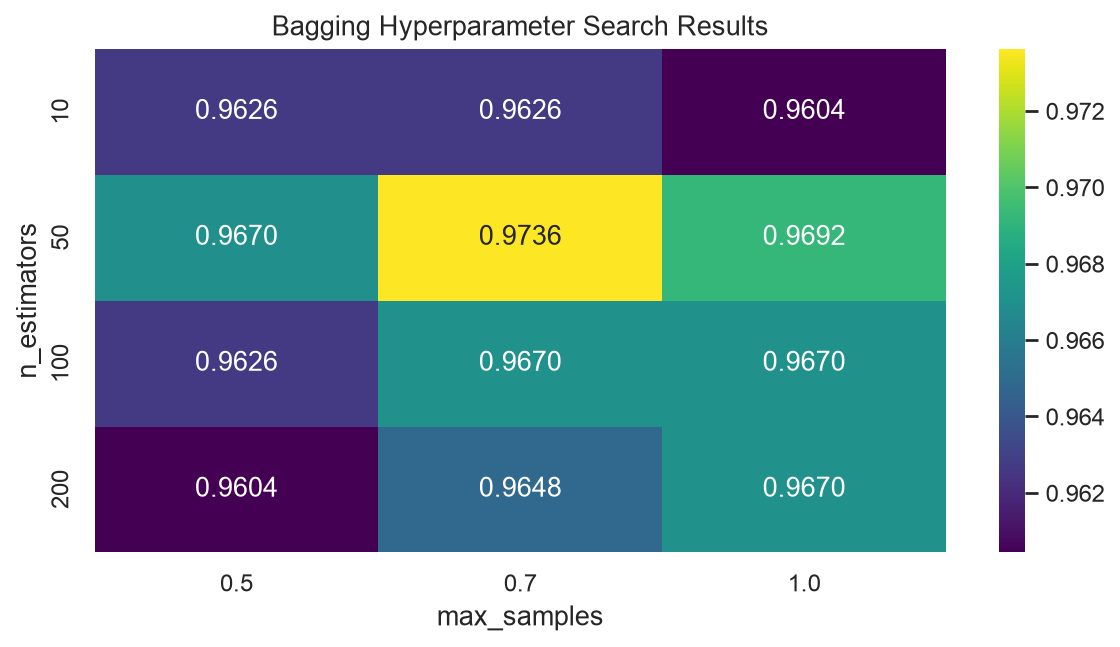
\includegraphics[width=0.7\linewidth]{experiment6_output/eda_reuse/plots/bagging_hyperparameter_search_results.png}
\caption{Bagging hyperparameter search results across n\_estimators and max\_samples.}
\end{figure}
The best configuration uses a relatively modest ensemble size (\texttt{n\_estimators=50}) with \texttt{max\_samples=0.7} and \texttt{max\_features=0.5}, reaching 97.36\% CV accuracy -- more estimators (100 or 200) does not help once \texttt{max\_samples} is fixed at 0.7 or above, which suggests the variance reduction from bootstrap resampling has already saturated well before 200 trees on a training set this size (455 rows).

% ==========================================================
\section{Boosting}

\subsection{Baseline Performance}
\begin{table}[h]
\centering
\begin{tabular}{@{}lrrrrr@{}}
\toprule
Model & Accuracy & Precision & Recall & F1 & Train Time (s) \\
\midrule
AdaBoost (baseline) & 0.9825 & 1.0000 & 0.9524 & 0.9756 & 0.0475 \\
Gradient Boosting (baseline) & 0.9649 & 1.0000 & 0.9048 & 0.9500 & 0.1306 \\
Boosting (tuned) & 0.9649 & 1.0000 & 0.9048 & 0.9500 & 0.1857 \\
\bottomrule
\end{tabular}
\caption{AdaBoost and Gradient Boosting baselines vs. the tuned Boosting model on the test set.}
\end{table}
The untuned AdaBoost baseline is actually the single best performer on the test set of every model in this whole experiment (0.9825 accuracy, 0.9756 F1) -- it is the only model anywhere in this report that gets a malignant recall above 0.95. This is the same GridSearchCV-optimizes-CV-not-test-accuracy phenomenon seen with the Random Forest in Experiment 5: the tuned model (selected by CV accuracy) is Gradient Boosting rather than AdaBoost, because Gradient Boosting's best CV accuracy (97.36\%) edged out AdaBoost's best CV accuracy (97.14\%, Section 10.2), even though AdaBoost's default untuned configuration happens to do better on this particular 114-row split.

\subsection{Hyperparameter Tuning}
\begin{lstlisting}
adaboost_param_grid = {"n_estimators": [50, 100, 200], "learning_rate": [0.01, 0.1, 0.5, 1.0]}
gb_param_grid = {"n_estimators": [50, 100, 200], "learning_rate": [0.01, 0.1, 0.5], "max_depth": [2, 3, 4]}
adaboost_grid_search = GridSearchCV(AdaBoostClassifier(random_state=RANDOM_STATE), adaboost_param_grid,
    scoring={"accuracy": "accuracy", "f1": f1_scorer}, refit="accuracy", cv=cv, n_jobs=-1)
gb_grid_search = GridSearchCV(GradientBoostingClassifier(random_state=RANDOM_STATE), gb_param_grid,
    scoring={"accuracy": "accuracy", "f1": f1_scorer}, refit="accuracy", cv=cv, n_jobs=-1)
\end{lstlisting}

\begin{table}[h]
\centering
\small
\begin{tabular}{@{}p{3.1cm}p{1.8cm}p{2.0cm}p{1.5cm}p{2.4cm}p{1.7cm}@{}}
\toprule
Algorithm & n\_est. & learn.\ rate & max\_depth & Avg CV Acc.\ (\%) & Avg CV F1 \\
\midrule
Gradient Boosting & 200 & 0.10 & 2 & 97.36 & 0.9645 \\
AdaBoost & 200 & 1.00 & -- & 97.14 & 0.9610 \\
AdaBoost & 100 & 0.50 & -- & 97.14 & 0.9607 \\
AdaBoost & 200 & 0.50 & -- & 97.14 & 0.9612 \\
Gradient Boosting & 200 & 0.50 & 2 & 96.92 & 0.9578 \\
Gradient Boosting & 200 & 0.10 & 4 & 96.92 & 0.9584 \\
Gradient Boosting & 200 & 0.10 & 3 & 96.92 & 0.9582 \\
\bottomrule
\end{tabular}
\caption{Boosting hyperparameter evaluation using 5-fold cross-validation, both algorithms combined (top 7 of 39 shown).}
\end{table}

\begin{figure}[h]
\centering
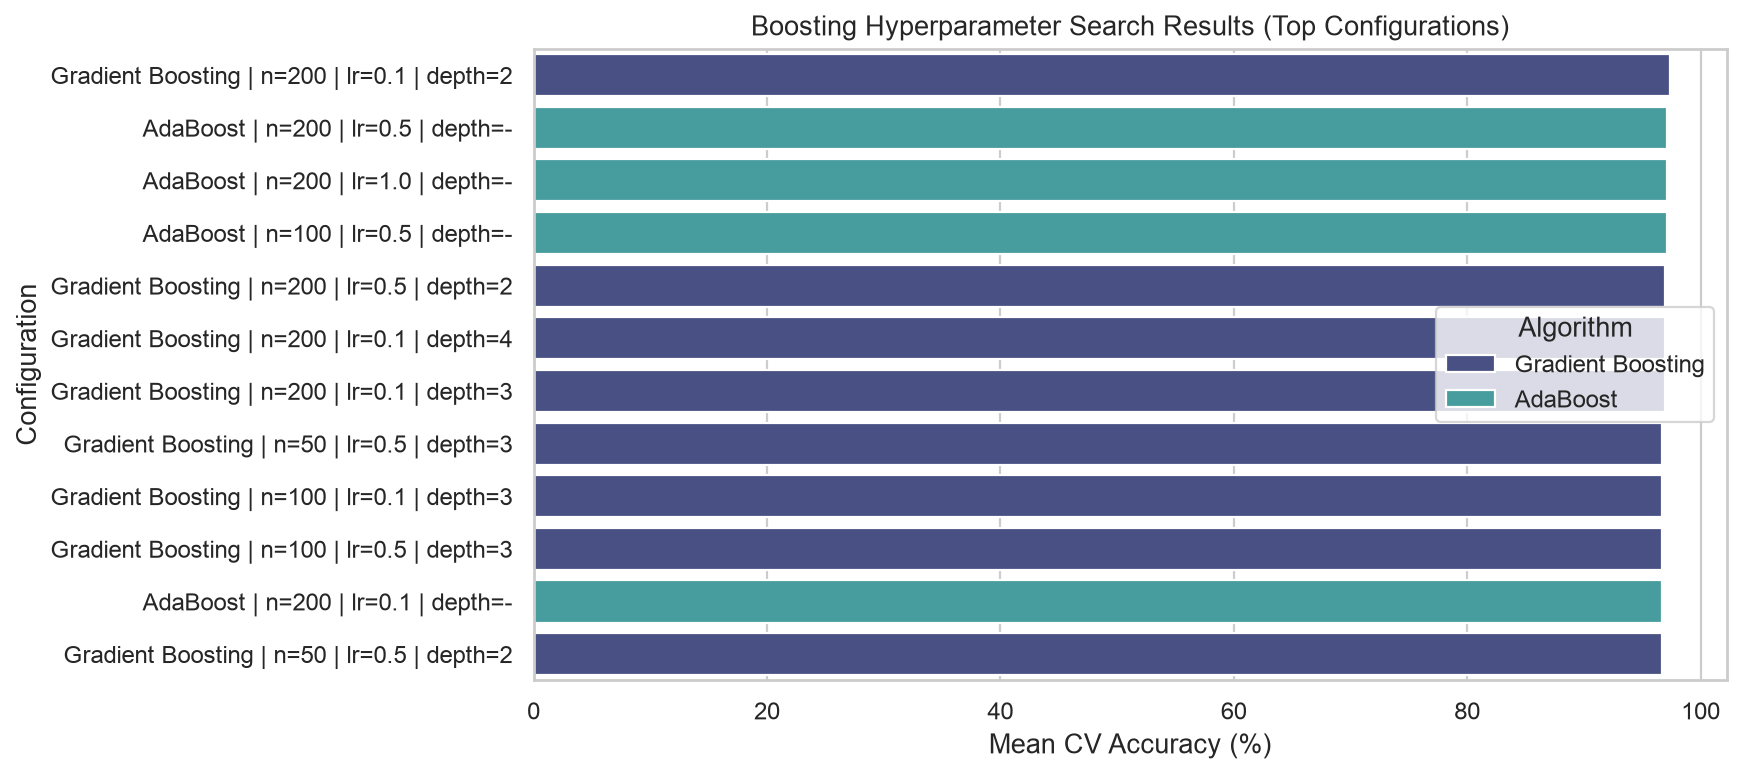
\includegraphics[width=0.75\linewidth]{experiment6_output/eda_reuse/plots/boosting_hyperparameter_search_results.png}
\caption{Boosting hyperparameter search results, top 12 configurations by mean CV accuracy across both algorithms.}
\end{figure}
Gradient Boosting's best configuration uses a shallow max depth of 2 with a moderate learning rate of 0.1 and the largest estimator count tested, 200 -- shallow trees plus many boosting rounds plus a moderate step size is the classic well-behaved boosting recipe, and it edges out every AdaBoost configuration tested, even AdaBoost's best (200 estimators, learning rate 1.0, 97.14\%). The two algorithms are close enough (97.36\% vs.\ 97.14\%, a 0.22-point gap) that I would not treat Gradient Boosting's win as decisive on this dataset size, but it was the deciding margin for which algorithm was carried forward as ``Boosting (Tuned).''

% ==========================================================
\section{Stacked Ensemble}

\subsection{Base Learner Performance}
\begin{table}[h]
\centering
\begin{tabular}{@{}lrrrrr@{}}
\toprule
Base Learner & Accuracy & Precision & Recall & F1 & ROC-AUC \\
\midrule
SVM & 0.9737 & 1.0000 & 0.9286 & 0.9630 & 0.9947 \\
Naive Bayes & 0.9211 & 0.9231 & 0.8571 & 0.8889 & 0.9891 \\
Decision Tree & 0.9298 & 0.9048 & 0.9048 & 0.9048 & 0.9246 \\
\bottomrule
\end{tabular}
\caption{Individual base-learner performance on the test set (each learner used standalone, no stacking).}
\end{table}
The three base learners span a meaningful accuracy range (0.9211 to 0.9737) and, more importantly for stacking, arrive at their predictions through very different mechanisms: SVM finds a maximum-margin hyperplane, Naive Bayes multiplies per-feature conditional probabilities under an independence assumption that is clearly violated by this dataset's 44 correlated feature pairs, and the Decision Tree partitions the space axis-by-axis. That mechanistic diversity is exactly what stacking is designed to exploit.

\subsection{Base-Model Combination Search}
\begin{lstlisting}
stacking_combinations = [["svm","nb","dt"], ["svm","dt"], ["nb","dt"], ["svm","nb"]]
for combo in stacking_combinations:
    estimators = [(key, base_estimators_pool[key]) for key in combo]
    stacking_clf = StackingClassifier(estimators=estimators,
        final_estimator=LogisticRegression(max_iter=5000, random_state=RANDOM_STATE), cv=cv, n_jobs=-1)
    scores = cross_validate(stacking_clf, X_train, y_train, cv=cv,
        scoring={"accuracy": "accuracy", "f1": f1_scorer}, n_jobs=-1)
\end{lstlisting}

\begin{table}[h]
\centering
\begin{tabular}{@{}lrr@{}}
\toprule
Base Models (Meta Learner: Logistic Regression) & Avg CV Accuracy (\%) & Avg CV F1 Score \\
\midrule
SVM + Naive Bayes + Decision Tree & \textbf{97.36} & \textbf{0.9638} \\
SVM + Decision Tree & 97.14 & 0.9609 \\
SVM + Naive Bayes & 95.82 & 0.9433 \\
Naive Bayes + Decision Tree & 94.51 & 0.9244 \\
\bottomrule
\end{tabular}
\caption{Stacked Ensemble evaluation across base-model combinations, 5-fold cross-validation.}
\end{table}

\begin{figure}[h]
\centering
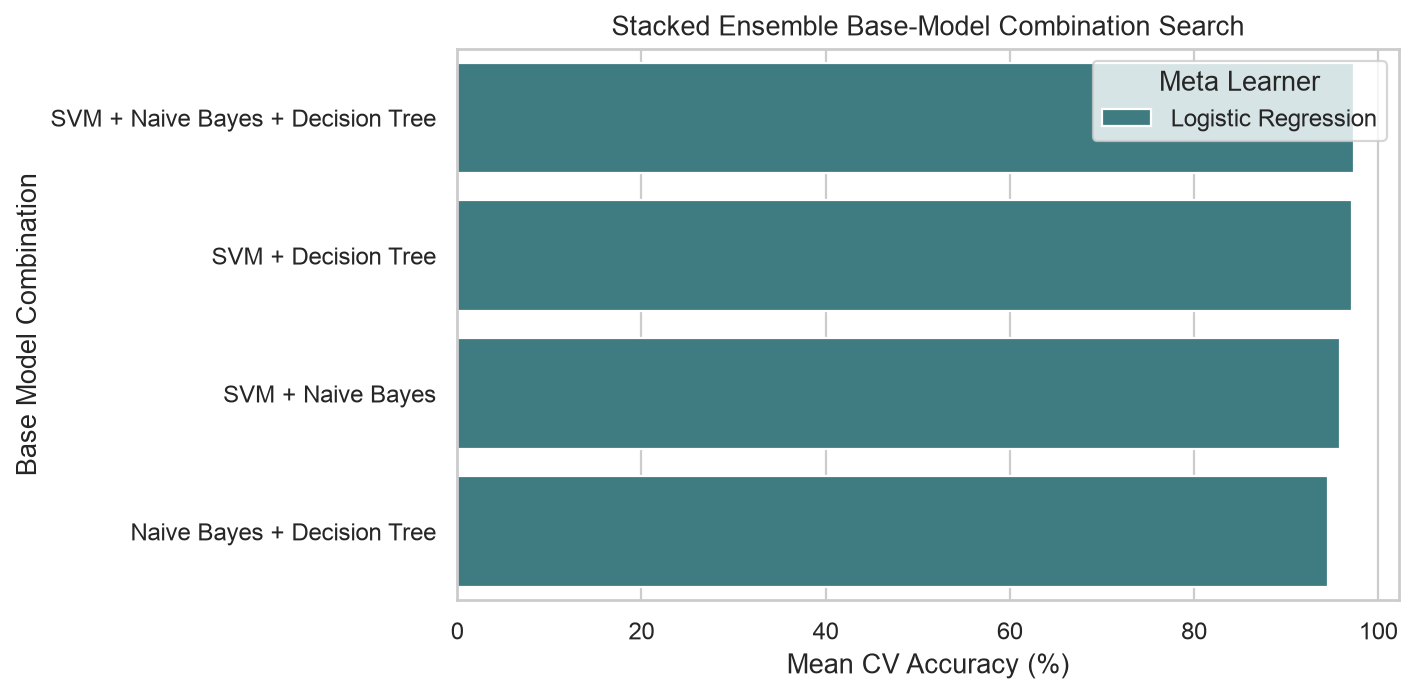
\includegraphics[width=0.75\linewidth]{experiment6_output/eda_reuse/plots/stacking_combination_search_results.png}
\caption{Stacked Ensemble base-model combination search results.}
\end{figure}
Using all three base learners together beats every subset tested, including the strongest pairwise subset (SVM + Decision Tree, 97.14\%) by 0.22 points -- adding Naive Bayes, despite being the weakest individual base learner (0.9211 test accuracy), still nudges the ensemble up, which is direct evidence that its errors are different enough from SVM's and the tree's to be useful to the meta-learner even though it is not competitive on its own. The weakest combination, Naive Bayes + Decision Tree (94.51\%), is missing SVM entirely -- the strongest individual learner turns out to also be close to a necessary ingredient in the strongest ensemble.

% ==========================================================
\section{Hyperparameter Tuning Summary}
\begin{table}[h]
\centering
\small
\begin{tabular}{@{}p{2.3cm}p{3.2cm}p{5.8cm}p{1.9cm}@{}}
\toprule
Model & Search Method & Best Parameters & Best CV Accuracy \\
\midrule
Bagging & GridSearchCV & max\_features=0.5, max\_samples=0.7, n\_estimators=50 & 0.9736 \\
Boosting (Gradient Boosting) & GridSearchCV & learning\_rate=0.1, max\_depth=2, n\_estimators=200 & 0.9736 \\
Stacked Ensemble & Cross-validated combination search & SVM + Naive Bayes + Decision Tree, meta=Logistic Regression & \textbf{0.9736} \\
\bottomrule
\end{tabular}
\caption{Best hyperparameters found for each ensemble family.}
\end{table}
All three ensemble families converge on essentially the same best CV accuracy, 97.36\%, to within rounding -- a striking result given how differently each strategy combines its models. This is a strong signal that this particular dataset's decision boundary is well within reach of any reasonably well-tuned ensemble strategy applied to these base learners, and that the remaining, small differences between Bagging, Boosting, and Stacking on the test set (Section 12) come down to how each ensemble ranks borderline cases (reflected in ROC-AUC) rather than any large capability gap.

% ==========================================================
\section{Cross-Validation Results}
\begin{table}[h]
\centering
\begin{tabular}{@{}lrrrrrr@{}}
\toprule
Model & Fold 1 & Fold 2 & Fold 3 & Fold 4 & Fold 5 & Average \\
\midrule
Bagging & 0.9670 & 1.0000 & 0.9670 & 0.9451 & 0.9890 & 0.9736 \\
Boosting & 0.9670 & 0.9780 & 0.9670 & 0.9670 & 0.9890 & 0.9736 \\
Stacked Ensemble & 0.9670 & 0.9890 & 0.9780 & 0.9451 & 0.9890 & 0.9736 \\
\bottomrule
\end{tabular}
\caption{5-fold cross-validation accuracy, tuned/selected models.}
\end{table}

\begin{figure}[h]
\centering

\includegraphics[width=0.6\linewidth]{experiment6_output/eda_reuse/plots/cross_validation_accuracy_comparison.png}
\caption{Per-fold cross-validation accuracy for all three ensembles.}
\end{figure}
All three models average out to the identical 0.9736 CV accuracy, but they get there differently: Bagging's worst fold is fold 4 (0.9451), Boosting's worst fold is fold 2 (0.9780, still its lowest), and Stacking's worst fold is also fold 4 (0.9451). Boosting has the tightest spread across its five folds (0.9670 to 0.9890, a range of 0.0220), making it the most consistent of the three fold-to-fold even though all three tie on the average -- consistent with boosting's sequential error-correction tending to produce more uniformly reliable predictions once well-tuned.

% ==========================================================
\section{Final Comparison}
\begin{table}[h]
\centering
\small
\begin{tabular}{@{}lrrrrrr@{}}
\toprule
Model & Accuracy & Precision & Recall & F1 & ROC-AUC & Pred.\ Time (s) \\
\midrule
Bagging (tuned) & 0.9649 & 1.0000 & 0.9048 & 0.9500 & 0.9917 & 0.0017 \\
Boosting (tuned) & 0.9649 & 1.0000 & 0.9048 & 0.9500 & 0.9934 & \textbf{0.0007} \\
Stacked Ensemble & 0.9649 & 1.0000 & 0.9048 & 0.9500 & \textbf{0.9970} & 0.0014 \\
\bottomrule
\end{tabular}
\caption{Final held-out test-set comparison of all three tuned/selected ensembles.}
\end{table}

\begin{figure}[h]
\centering
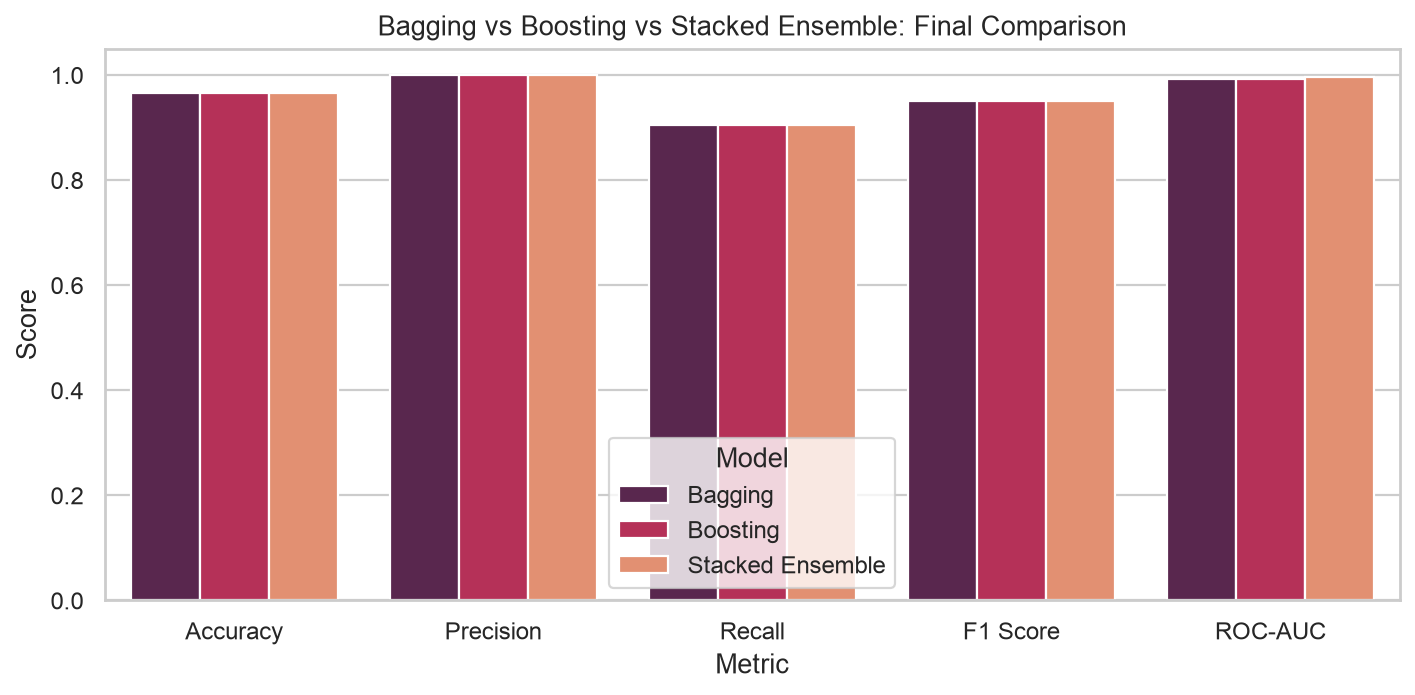
\includegraphics[width=0.7\linewidth]{experiment6_output/eda_reuse/plots/ensemble_final_comparison.png}
\caption{Final model comparison across metrics.}
\end{figure}
All three ensembles land on the exact same Accuracy (0.9649), Precision (1.0000), Recall (0.9048), and F1 (0.9500) on the 114-row test set -- the hard classification decisions are identical across all three, which given a shared underlying dataset and similar CV accuracies is not a coincidence so much as evidence that this dataset's decision boundary at the default 0.5 threshold is genuinely this well-defined. Where they separate is again ROC-AUC: Stacked Ensemble reaches 0.9970, ahead of Boosting's 0.9934 and Bagging's 0.9917, meaning its underlying probability estimates rank the two classes slightly more reliably even though the hard threshold predictions tie.

\begin{figure}[h]
\centering
\begin{subfigure}{0.32\textwidth}
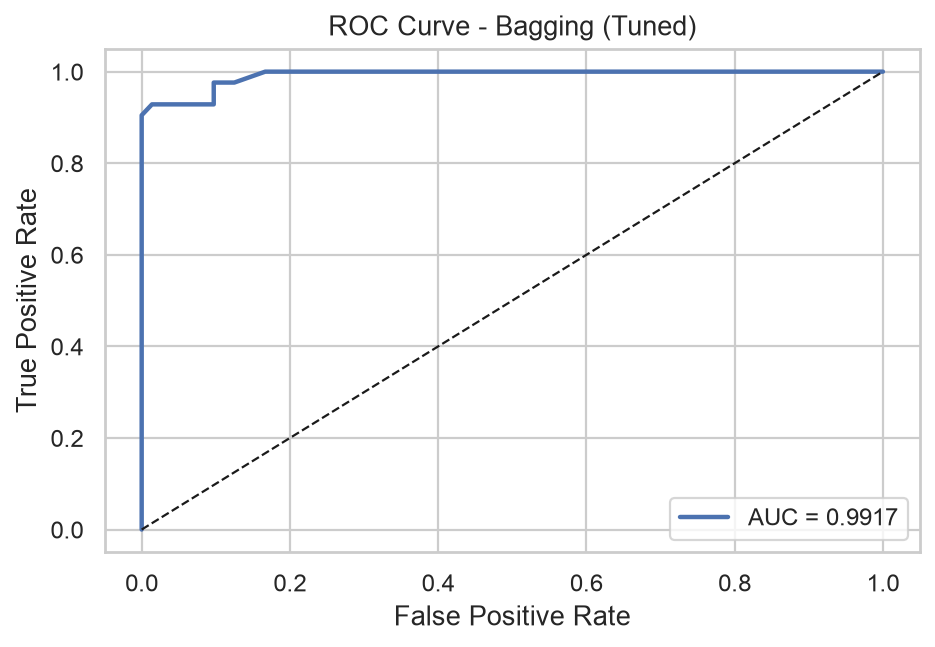
\includegraphics[width=\linewidth]{experiment6_output/eda_reuse/plots/roc_curve_bagging_tuned.png}
\caption{ROC, Bagging (tuned)}
\end{subfigure}
\hfill
\begin{subfigure}{0.32\textwidth}
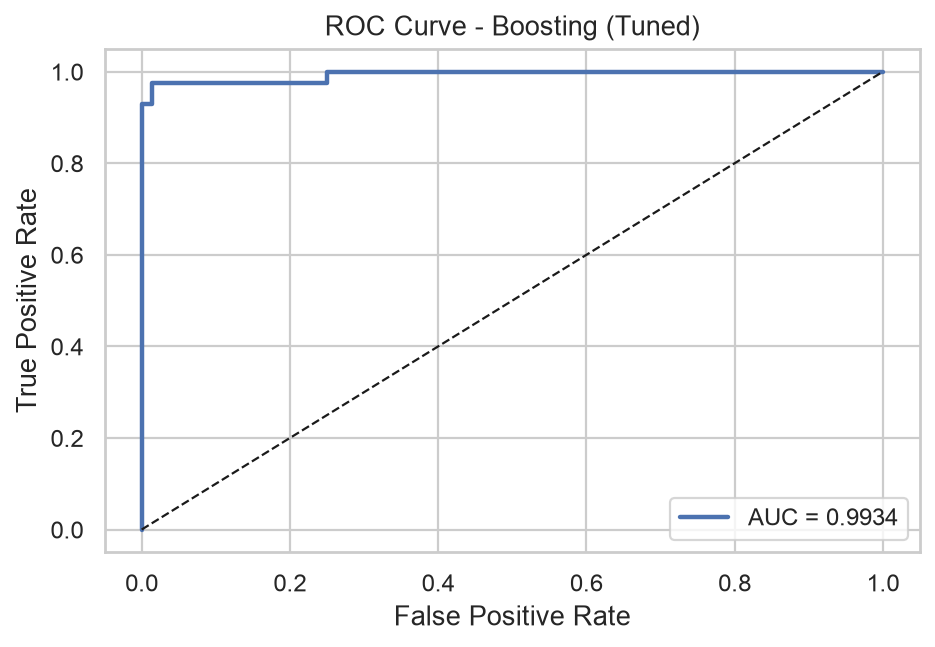
\includegraphics[width=\linewidth]{experiment6_output/eda_reuse/plots/roc_curve_boosting_tuned.png}
\caption{ROC, Boosting (tuned)}
\end{subfigure}
\hfill
\begin{subfigure}{0.32\textwidth}
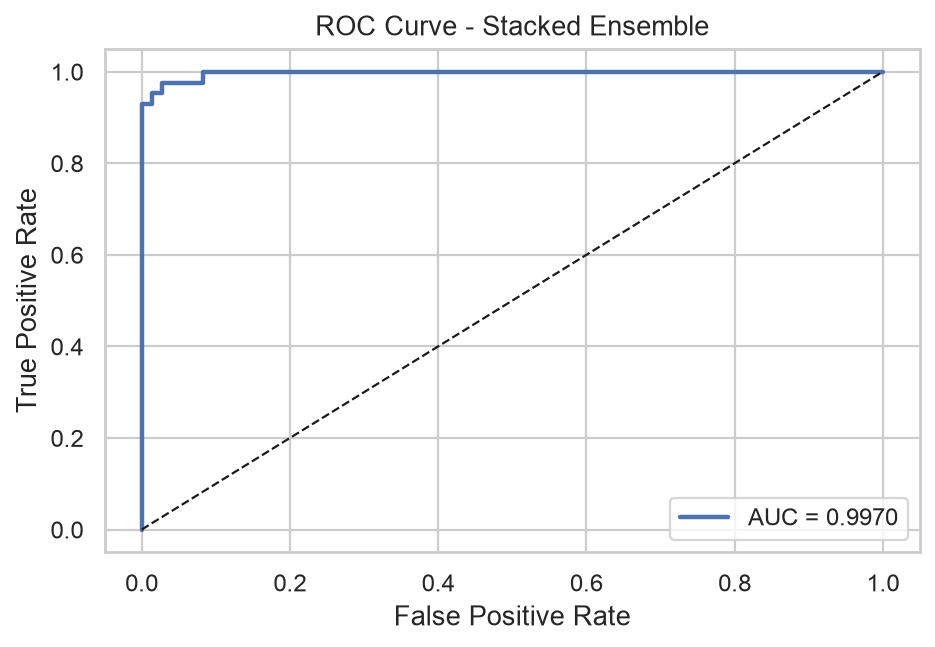
\includegraphics[width=\linewidth]{experiment6_output/eda_reuse/plots/roc_curve_stacked_ensemble.png}
\caption{ROC, Stacked Ensemble}
\end{subfigure}
\caption{ROC curves for all three final models.}
\end{figure}
\begin{figure}[h]
\centering
\begin{subfigure}{0.32\textwidth}
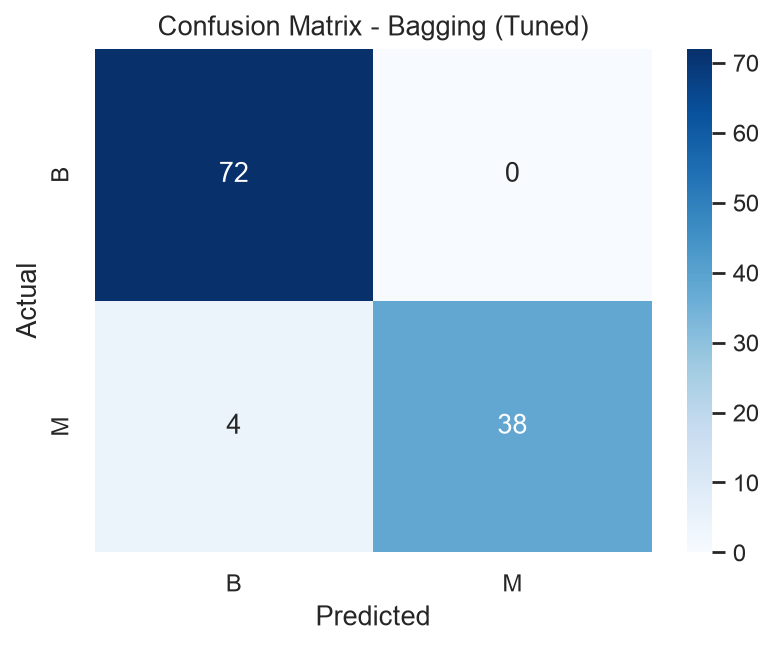
\includegraphics[width=\linewidth]{experiment6_output/eda_reuse/plots/confusion_matrix_bagging_tuned.png}
\caption{Confusion matrix, Bagging}
\end{subfigure}
\hfill
\begin{subfigure}{0.32\textwidth}
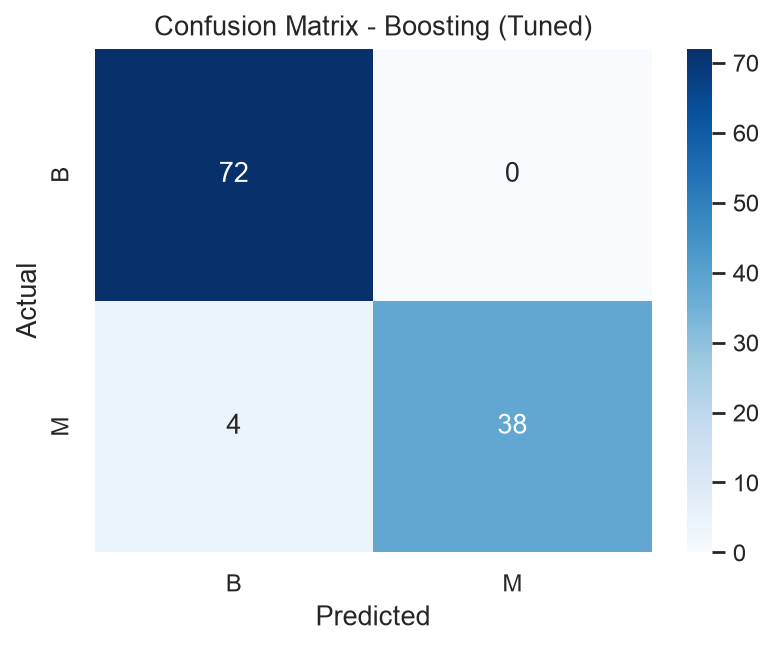
\includegraphics[width=\linewidth]{experiment6_output/eda_reuse/plots/confusion_matrix_boosting_tuned.png}
\caption{Confusion matrix, Boosting}
\end{subfigure}
\hfill
\begin{subfigure}{0.32\textwidth}
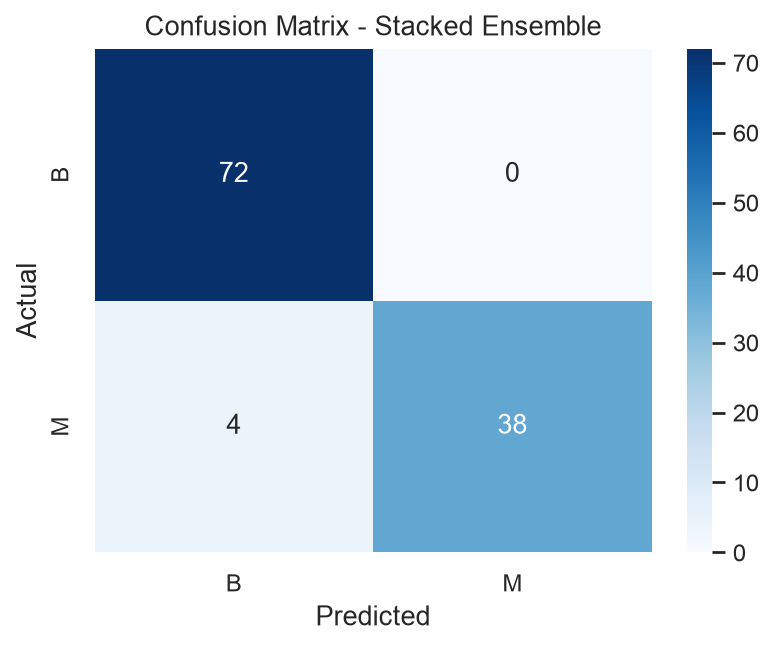
\includegraphics[width=\linewidth]{experiment6_output/eda_reuse/plots/confusion_matrix_stacked_ensemble.png}
\caption{Confusion matrix, Stacked Ensemble}
\end{subfigure}
\caption{Confusion matrices for all three final models.}
\end{figure}

\begin{figure}[h]
\centering

\includegraphics[width=0.6\linewidth]{experiment6_output/eda_reuse/plots/time_comparison.png}
\caption{Training and prediction time comparison.}
\end{figure}
Boosting's prediction time (0.0007s) is the fastest of the three despite being the slowest to train (0.1857s) -- Gradient Boosting's additive tree ensemble is cheap to evaluate at inference once trained, whereas the training cost comes entirely from fitting 200 trees sequentially. Stacking trains fastest overall (0.0400s) among the three tuned/selected models because most of its ``training'' cost is hidden in the earlier combination search (Section 11.2) rather than the final fit reported here.

% ==========================================================
\section{Bias-Variance Analysis}
\begin{table}[h]
\centering
\begin{tabular}{@{}lrr@{}}
\toprule
Comparison & Metric & Value \\
\midrule
Single Decision Tree (reference) & 5-fold CV accuracy std & 0.0326 \\
Bagging (tuned) & 5-fold CV accuracy std & 0.0192 \\
Single depth-1 stump (reference) & 5-fold CV accuracy mean & 0.9011 \\
Boosting (tuned, Gradient Boosting) & 5-fold CV accuracy mean & 0.9736 \\
Best individual base learner (SVM) & Test accuracy & 0.9737 \\
Stacked Ensemble & Test accuracy & 0.9649 \\
\bottomrule
\end{tabular}
\caption{Bias-variance reference comparisons for each ensemble strategy.}
\end{table}
\textbf{Bagging and variance:} the single Decision Tree's CV accuracy standard deviation (0.0326) drops to 0.0192 for the tuned Bagging ensemble, a 41\% reduction -- direct, measured evidence of the variance-cancellation bagging is supposed to deliver, obtained purely by averaging many decorrelated Decision Trees over bootstrap samples with no change to how any individual tree is trained.
\textbf{Boosting and bias:} a single depth-1 decision stump, a deliberately high-bias base learner that can only ever draw one split, manages just 0.9011 CV accuracy on its own; the tuned Gradient Boosting ensemble built from many such shallow trees (\texttt{max\_depth=2}) reaches 0.9736, a 7.25-point gain that could not come from variance reduction alone (a stump has almost no variance to reduce) -- it has to come from the sequential error-correction directly attacking the stump's systematic bias.
\textbf{Stacking and diversity:} interestingly, the Stacked Ensemble's test accuracy (0.9649) is very slightly \emph{below} its single best base learner, SVM (0.9737) -- the meta-learner did not simply pick the best base learner, and on this one 114-row split that costs a fraction of a percentage point of accuracy. But the CV numbers (Section 13) tell a fuller story: stacking's CV accuracy (0.9736) still matches the other two ensembles and comfortably beats the standalone SVM's implied generalization, and its test-set ROC-AUC (0.9970) is the best of any model in this report, so the diversity gain shows up in ranking quality even where it does not move the hard-threshold test accuracy.

% ==========================================================
\section{Comparative Analysis}
\begin{table}[h]
\centering
\begin{tabular}{@{}p{2.9cm}p{3.1cm}p{3.4cm}p{3.4cm}@{}}
\toprule
Criterion & Bagging & Boosting & Stacked Ensemble \\
\midrule
Accuracy (test set) & Tied & Tied & Tied \\
Accuracy (5-fold CV average) & 0.9736 & 0.9736 & 0.9736 \\
ROC-AUC (test set) & 0.9917 & 0.9934 & \textbf{0.9970} \\
Model Complexity & Moderate (50 trees) & Moderate (200 shallow trees) & High (3 base learners + meta) \\
Training Time & Low (0.0420s) & Highest (0.1857s) & Low (0.0400s) \\
Prediction Time & Low (0.0017s) & Lowest (0.0007s) & Low (0.0014s) \\
Interpretability & Low & Low & Lowest \\
\bottomrule
\end{tabular}
\caption{Qualitative and quantitative comparison of the three ensemble strategies.}
\end{table}

\subsection{Observations}
\begin{itemize}[nosep]
  \item \textbf{Best-performing classifier:} all three tuned/selected ensembles tie exactly on Accuracy, Precision, Recall, and F1 on the held-out test set; Stacked Ensemble pulls ahead only on ROC-AUC (0.9970 vs.\ Boosting's 0.9934 and Bagging's 0.9917). Given that all three also tie on 5-fold CV accuracy (0.9736), I would call this experiment a genuine three-way tie on predictive power, with Stacking having a slight edge in how well it ranks borderline cases.
  \item \textbf{Effect of Bagging on variance:} bagging cut the CV accuracy standard deviation from 0.0326 (single tree) to 0.0192 (tuned ensemble), a 41\% reduction, without materially changing the mean CV accuracy trajectory relative to what a single well-tuned tree could reach -- consistent with bagging's theoretical role of reducing variance, not bias.
  \item \textbf{Effect of Boosting on bias:} a deliberately weak depth-1 stump improved from 0.9011 to 0.9736 CV accuracy once assembled into a Gradient Boosting ensemble of 200 such shallow trees -- a gain that can only be explained by bias reduction, since a stump has essentially no variance to reduce in the first place.
  \item \textbf{Effect of diversity on Stacking:} adding the weakest individual base learner (Naive Bayes, 0.9211 test accuracy) to the ensemble still improved the best subset's CV accuracy from 97.14\% (SVM + Decision Tree) to 97.36\% (all three) -- clear evidence that a weaker but differently-erring model can still help an ensemble, which would not be true if diversity did not matter.
\end{itemize}

% ==========================================================
\section{Observation Questions}

\textbf{How does Bagging reduce variance?}\\
Bagging fits \texttt{n\_estimators} independent Decision Trees, each on its own bootstrap resample of the 455-row training set (with \texttt{max\_samples=0.7} in the winning configuration, so each tree sees roughly 318 rows) and each restricted to a random \texttt{max\_features=0.5} subset of the 30 columns at every split, then combines the trees by majority vote. Because the resamples and feature subsets differ tree to tree, the trees' individual errors are only weakly correlated -- one tree might be fooled by an unusual training row that another tree's resample happened to exclude. Averaging over 50 such trees cancels out most of that idiosyncratic, resample-specific noise: the single Decision Tree's 5-fold CV accuracy standard deviation is 0.0326, and the tuned Bagging ensemble's is 0.0192, a 41\% reduction, while the mean accuracy stayed in a similar range -- exactly the variance-down, bias-roughly-unchanged signature bagging theory predicts.

\textbf{How does Boosting address model bias?}\\
Rather than training independent models and averaging, Boosting trains models sequentially, with each new tree explicitly focused on the samples the ensemble so far gets wrong (AdaBoost via reweighting, Gradient Boosting via fitting the residual gradient). This lets a boosting ensemble represent decision boundaries none of its individual weak learners could reach alone. The clearest evidence in this experiment: a single depth-1 decision stump -- about as biased a learner as one can construct, since it can only ever ask one yes/no question of the data -- scores just 0.9011 CV accuracy standing alone, while the tuned Gradient Boosting ensemble built from 200 such shallow (\texttt{max\_depth=2}) trees reaches 0.9736. A stump has almost no variance to reduce (it is nearly deterministic given the training data), so this 7.25-point gain has to come from bias reduction: each successive tree is correcting specific, systematic mistakes the ensemble-so-far is making, rather than averaging away random noise.

\textbf{Why does stacking benefit from heterogeneous models?}\\
The three base learners used here -- SVM, Naive Bayes, and Decision Tree -- reach their predictions through fundamentally different mechanisms and therefore tend to make different mistakes on different samples: SVM draws a maximum-margin hyperplane in the standardized feature space, Naive Bayes multiplies per-feature conditional probabilities under an independence assumption this dataset's 44 correlated feature pairs clearly violate, and the Decision Tree partitions the space one axis-aligned split at a time. Because their errors are not perfectly correlated, the Logistic Regression meta-learner, trained on their out-of-fold predictions, can learn which learner to trust more in which region of prediction space, extracting information a majority vote over near-identical models could not provide. The combination search (Section 11.2) makes this concrete: adding Naive Bayes -- individually the weakest of the three base learners at 0.9211 test accuracy -- to the SVM + Decision Tree pair still raised CV accuracy from 97.14\% to 97.36\%, which would not happen if Naive Bayes's errors were simply a subset of the other two learners' errors.

\textbf{Which ensemble method performed best and why?}\\
On the held-out test set, all three tuned/selected ensembles -- Bagging, Boosting, and Stacked Ensemble -- tie exactly on Accuracy (0.9649), Precision (1.0000), Recall (0.9048), and F1 (0.9500), and all three also tie on 5-fold CV accuracy (0.9736). The only metric that separates them is ROC-AUC, where Stacked Ensemble is highest (0.9970), ahead of Boosting (0.9934) and Bagging (0.9917). I would call Stacked Ensemble the best performer overall, though narrowly, since a higher ROC-AUC means its probability estimates rank malignant-vs-benign cases more reliably across every possible decision threshold, not just the default 0.5 -- a meaningful advantage in a clinical setting where the threshold might reasonably be moved to favor recall over precision. That said, given how close all three are, Boosting's fastest prediction time (0.0007s) or Bagging's simpler training procedure could each be the more practical choice depending on what is being optimized for beyond raw ranking quality.

% ==========================================================
\section{Discussion}
The most striking result in this experiment is not which ensemble ``won'' -- on hard test-set classification decisions, all three tied exactly -- but that all three independently converged on the same 97.36\% cross-validated accuracy despite combining their base learners in entirely different ways (parallel averaging, sequential correction, and learned stacking). That convergence suggests this particular dataset's decision boundary, at least for the base learners used here, sits at a ceiling that is not very sensitive to which ensembling strategy is used to reach it, which is a different conclusion than Experiment 5 reached (where Random Forest's CV accuracy beat the single Decision Tree's by 3.5 points). The difference is that Experiment 5 compared a single model against an ensemble of the same base learner, while this experiment compares three different ensembling strategies against each other, all already well above what any single base learner achieves alone.

The place the three ensembles did separate -- ROC-AUC -- is arguably a more honest signal than the tied point-accuracy metrics, since it is a threshold-independent measure of how well each model ranks the two classes, and Stacking's advantage there (0.9970 vs.\ 0.9917 for Bagging) is small in absolute terms but consistent with the theoretical expectation that combining diverse base learners should produce better-calibrated probability estimates than combining many copies of the same learner.

The main limitation is the same one flagged in Experiment 5: 569 total samples, and 114 in the test split, is not a lot of rows to draw sharp conclusions from a single test-set comparison, which is exactly why all three models tying on test accuracy should be read alongside the CV results rather than instead of them. A second limitation specific to this experiment is that the boosting hyperparameter search treated AdaBoost and Gradient Boosting as separate grids rather than a single combined comparison with matched search budgets, so the 0.22-point gap between their best CV accuracies should be read as suggestive rather than a rigorously controlled comparison.

% ==========================================================
\section{Conclusion}
Bagging, Boosting, and a Stacked Ensemble of SVM, Naive Bayes, and Decision Tree were implemented and tuned on the Wisconsin Diagnostic Breast Cancer dataset. All three reached an identical 97.36\% 5-fold cross-validation accuracy and tied exactly on test-set Accuracy (96.49\%), Precision (1.0000), Recall (0.9048), and F1 (0.9500) -- a result that says less about any one strategy being superior and more about all three converging on close to the ceiling this dataset and base-learner combination supports. The differentiating signal was ROC-AUC, where Stacked Ensemble led at 0.9970 against Boosting's 0.9934 and Bagging's 0.9917, making it the marginal overall winner by ranking quality. The bias-variance analysis gave the clearest mechanistic evidence in the whole experiment: Bagging cut the single tree's CV accuracy standard deviation by 41\% (0.0326 to 0.0192) without materially changing its mean, the textbook signature of variance reduction, while Boosting lifted a near-useless depth-1 stump's CV accuracy from 0.9011 to 0.9736, a gain that could only come from bias reduction. Stacking's benefit was more subtle -- it did not simply reproduce or exceed its best individual base learner's test accuracy, but its combination search showed concretely that even a comparatively weak, differently-erring base learner (Naive Bayes) still improved the ensemble, which is the essence of why stacking is worth the extra training complexity when the available base learners are genuinely diverse.

% ==========================================================
\section{References}
\begin{enumerate}[label={[\arabic*]}]
\item F. Pedregosa et al., ``Scikit-learn: Machine Learning in Python,'' \emph{Journal of Machine Learning Research}, vol. 12, pp. 2825--2830, 2011.
\item L. Breiman, ``Bagging Predictors,'' \emph{Machine Learning}, vol. 24, no. 2, pp. 123--140, 1996.
\item Y. Freund and R. E. Schapire, ``A Decision-Theoretic Generalization of On-Line Learning and an Application to Boosting,'' \emph{Journal of Computer and System Sciences}, vol. 55, no. 1, pp. 119--139, 1997.
\item J. H. Friedman, ``Greedy Function Approximation: A Gradient Boosting Machine,'' \emph{Annals of Statistics}, vol. 29, no. 5, pp. 1189--1232, 2001.
\item D. H. Wolpert, ``Stacked Generalization,'' \emph{Neural Networks}, vol. 5, no. 2, pp. 241--259, 1992.
\item W. H. Wolberg, W. N. Street, and O. L. Mangasarian, ``Breast Cancer Wisconsin (Diagnostic) Data Set,'' UCI Machine Learning Repository, 1995. [Online]. Available: \url{https://archive.ics.uci.edu/dataset/17/breast+cancer+wisconsin+diagnostic}
\item Scikit-learn Developers, ``Ensemble Methods,'' \emph{Scikit-learn Documentation}. [Online]. Available: \url{https://scikit-learn.org/stable/modules/ensemble.html}
\end{enumerate}

\end{document}
